%%% LaTeX Template
%%% This template can be used for both articles and reports.
%%%
%%% Copyright: http://www.howtotex.com/
%%% Date: February 2011

%%% Preamble
\documentclass[paper=a4, fontsize=11pt]{scrartcl}	% Article class of KOMA-script with 11pt font and a4 format
\usepackage[margin=0.7in]{geometry}
\usepackage[english]{babel}															% English language/hyphenation
\usepackage[protrusion=true,expansion=true]{microtype}				% Better typography
\usepackage{amsmath,amsfonts,amsthm}										% Math packages
%\usepackage{color,transparent}													% If you use color and/or transparency
\usepackage[hang, small,labelfont=bf,up,textfont=it,up]{caption}	% Custom captions under/above floats
\usepackage{epstopdf}																	% Converts .eps to .pdf
\usepackage{subfig}																		% Subfigures
\usepackage{booktabs}																	% Nicer tables
\usepackage[pdftex]{graphicx}

%%% Advanced verbatim environment
\usepackage{verbatim}
\usepackage{fancyvrb}
\DefineShortVerb{\|}								% delimiter to display inline verbatim text


%%% Custom sectioning (sectsty package)
\usepackage{sectsty}								% Custom sectioning (see below)
\allsectionsfont{%									% Change font of al section commands
	\usefont{OT1}{bch}{b}{n}%					% bch-b-n: CharterBT-Bold font
%	\hspace{15pt}%									% Uncomment for indentation
	}

\sectionfont{%										% Change font of \section command
	\usefont{OT1}{bch}{b}{n}%					% bch-b-n: CharterBT-Bold font
	\sectionrule{0pt}{0pt}{-5pt}{0.8pt}%	% Horizontal rule below section
	}


%%% Custom headers/footers (fancyhdr package)
\usepackage{fancyhdr}
\pagestyle{fancyplain}
\fancyhead{}														% No page header
\fancyfoot[C]{\thepage}										% Pagenumbering at center of footer
\renewcommand{\headrulewidth}{0pt}				% Remove header underlines
\renewcommand{\footrulewidth}{0pt}				% Remove footer underlines
\setlength{\headheight}{13.6pt}

%%% Equation and float numbering
\numberwithin{equation}{section}															% Equationnumbering: section.eq#
\numberwithin{figure}{section}																% Figurenumbering: section.fig#
\numberwithin{table}{section}

\usepackage[parfill]{parskip}
\usepackage{float}
\usepackage{hyperref}
\usepackage[numbers]{natbib}															% Tablenumbering: section.tab#


%%% Title
\title{
	\vspace{-0.5in} 	\usefont{OT1}{bch}{b}{n}
	 SE31520 Developing Internet Applications: CS Alumni Assignment\
}

%Authors
\author{
	\usefont{OT1}{bch}{m}{n} Samuel Jackson
	\\ \usefont{OT1}{bch}{m}{n} University Of Aberystwyth
	\\   \texttt{slj11@aber.ac.uk}
}

\date{\today}

\begin{document}

\maketitle
\clearpage

\section{Introduction}
This report documents the assessed project for the SE31520 module Developing Internet-Based Applications. For this assignment I chose to create a RESTful client application which communicates with the CS alumni site outlined in the brief. The RESTful client is implemented in the Python language as a basic command line utility. The client uses the requests library \cite{libraryRequests} to create HTTP requests to the CSA site. The command line interface has been created using the click library \cite{libraryClick}. The basic functionality of the client application replicates almost all of the existing CRUD operations available through the CSA site. 

I have made very little changes to the server side of the site. The major changes regarding the existing work is the addition of a lot more testing for both controllers, enabling SSL support and adding OAuth 2.0 \cite{rfc6749} support via the Doorkeeper gem \cite{libraryDoorkeeper}. The client and server together implement support for the resource owner password credentials grant \cite{rfc6749resourceOwner} including refresh token support. I have also added some additional routing aliases for the resource operations on the server for convenience. Finally, I also added the ability to search for broadcasts via content or user ID. This is implemented identically to the user search functionality.

The rest of the report is structured as follows: In section \ref{sec:requirements} briefly outlines the use cases for both the CSA site and client. Section \ref{sec:design} gives an overview of the architecture of the system for both the CSA server and the client application. Section \ref{sec:testing} outlines my approach to testing both components of the system and section \ref{sec:evaluation} provides an analysis of the project; drawing conclusions on the work produced and what could have been done better in hindsight.

\section{Requirements}
\label{sec:requirements}
The user stories for the CS alumni site have already been outlined in the requirements document provided as part of the assignment brief. The use cases are essentially the same for both the CSA site and the RESTful client application. Broadly speaking there are three different kinds of users. Guests are unregistered users who can only view the website home page and the login page. In the client application a user must login before they can perform any actions on the site. Registered uses who are not admins can view and update details about their account. Admins can perform all the actions of a regular user, but can additionally carry out CRUD operations on all users and search for users in the system. Furthermore admins can also view, create and delete (records of) broadcasts to all users of the site through a variety of media. The use case diagram in figure \ref{fig:use-cases} summarises the major actions that can be performed from via the site and the RESTful client.

\begin{figure}[H]
\centering
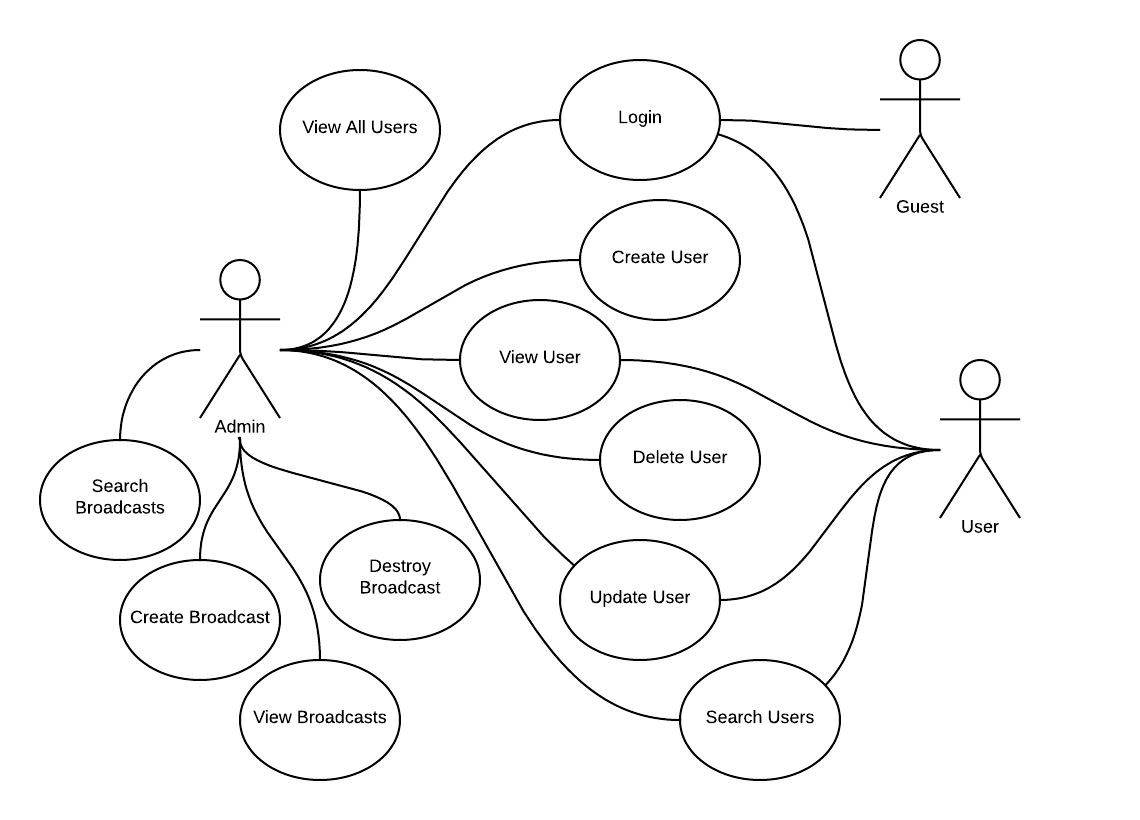
\includegraphics[width=0.7\textwidth]{img/use_cases.png}
\caption{Shows the use cases for the CSA site. Guests not registered in the with the site can only attempt to login. Users can login to the site and view and edit themselves. Admins can do all of these actions, but can also create users and view, edit and delete any user. Admins may also create and view broadcasts sent from the site, as well as destroy records of existing records. Admins may also search for users and broadcasts}
\label{fig:use-cases}
\end{figure}

\section{Design}
\label{sec:design}
This section outlines the design of both the existing server side application which the client application communicates with and the client application itself.

\subsection{Server Architecture}
\label{subsec:server-architecture}
The CSA website uses the Ruby on Rails web framework which uses a model-view-controller architecture to structure its programs. In the Rails framework models follow the active record pattern and have a mapping to a table in the database. Controller objects provide definitions for the CRUD operations that can be performed on models with the site. Finally, the views in a Rails application are usually defined by embedded ruby files which build a dynamically created view of the application.

The CS alumni applications has multiple instances of models, views and controllers. The two main models are the Users object and the Broadcasts object. A User object defines a record for a registered site user. Every registered user also has an instance of a UserDetails model. This model is stored in a separate table in the database to the User model and handles a user's login and password details. Broadcasts are messages that can be sent to users of the site by administrators through a variety of feeds (Email, Twitter, RSS etc.). Currently the only communication channels supported by Broadcasts are email and twitter.

In Rails application the controllers handle the incoming HTTP requests from the web. In the CS alumni site six controller classes defined. The first is a generic application controller that extends the Rails version of an application contoller. The other controllers further extend this controller in turn. There is one controller each for the User and Broadcast objects which are responsible for performing CRUD operations on them. There is also a controller for handling the creation of a new user session when a user logs in from the ``human'' version of the site. There is also the (empty) home controller which currently just shows the index page. I have also added a basic controller to add support for HTCPCP \cite{rfc2324htcpcp}.

In addition to the original database design the Doorkeeper OAuth gem automatically generates a number of other tables that were not part of the original design. The current client-server system only uses one of these new tables. The oauth\_access\_tokens table is where access tokens granted to users are stored. Each record has a resource owner ID which is a foreign key to an entry in the user details table.

\begin{figure}[H]
\centering
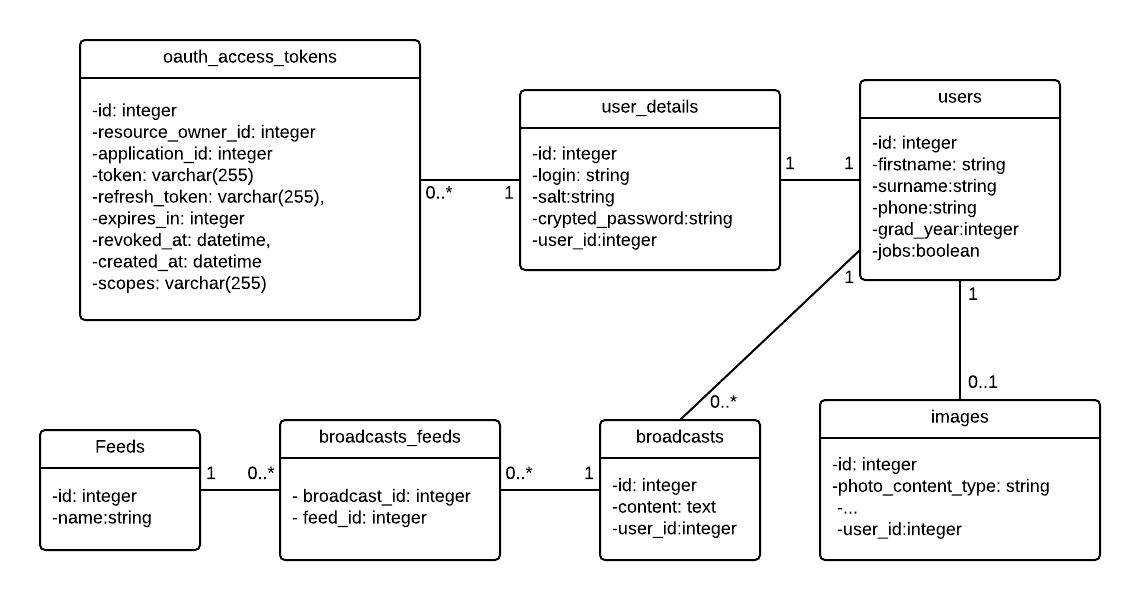
\includegraphics[width=0.8\textwidth]{img/database_design.png}
\caption{The database design of the CSA site. This is based on the original design by Chris Loftus. The only addition here is an extra table for the oauth\_access\_tokens, linked to a specific user. This table was automatically generated by Doorkeeper. Additional tables were also auto generated, but have been omitted.}
\label{fig:database-design}
\end{figure}

\begin{figure}[H]
\centering
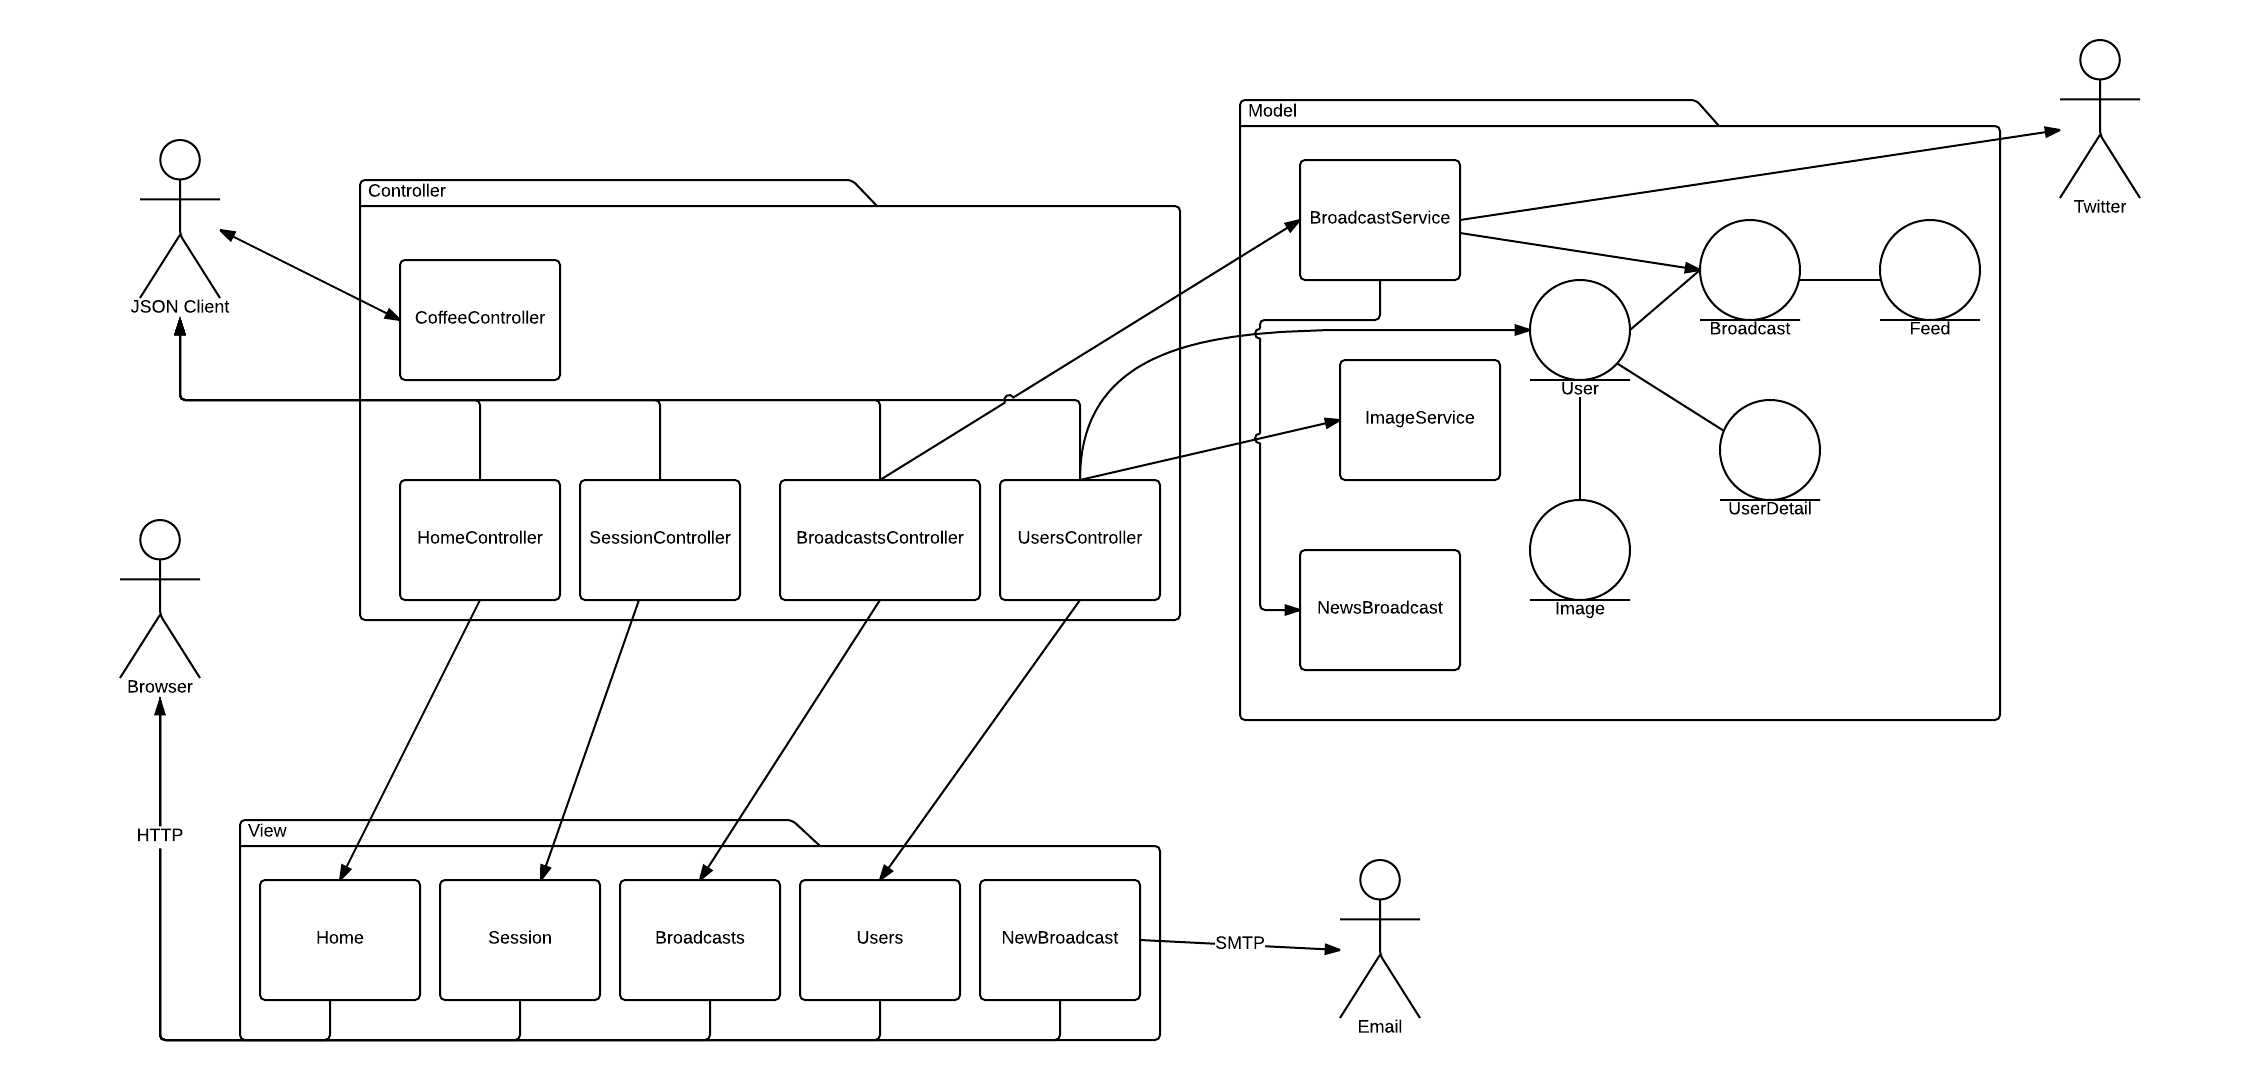
\includegraphics[width=1.1\textwidth]{img/entity_relationship.png}
\caption{Shows a class diagram overview of the system. This is based on the original design by Chris Loftus. The only addition to the original design is the CoffeeController for handling very basic HTCPCP requests.}
\label{fig:entity-realtionship}
\end{figure}

\subsection{Client Architecture}
\label{subsec:client-architecture}
The client side of the application is a lightweight wrapper to the requests library \citep{libraryRequests}. The core class driving the design is the RequestsHandler. This handles setting up HTTP requests to one of the predefined end points of the server application. In order to add OAuth 2.0 resource owner support the RequestHandler is extended by an additional class called the OAuth2ResourceOwner. This provides additional functionality for automatically refreshing expired OAuth tokens. Additional ``flows'' from OAuth 2.0 could also be implemented through such a mechanism in future development. The CsaAPI class has an instance of a RequestsHandler object and defines a collection of helper methods that make HTTP requests through the requests handler. Finally, the command line interface is defined as a collection of functions in command.py. This only utilises the CsaAPI and does not use the other classes directly (except the TokenCache).

\begin{figure}[H]
\centering
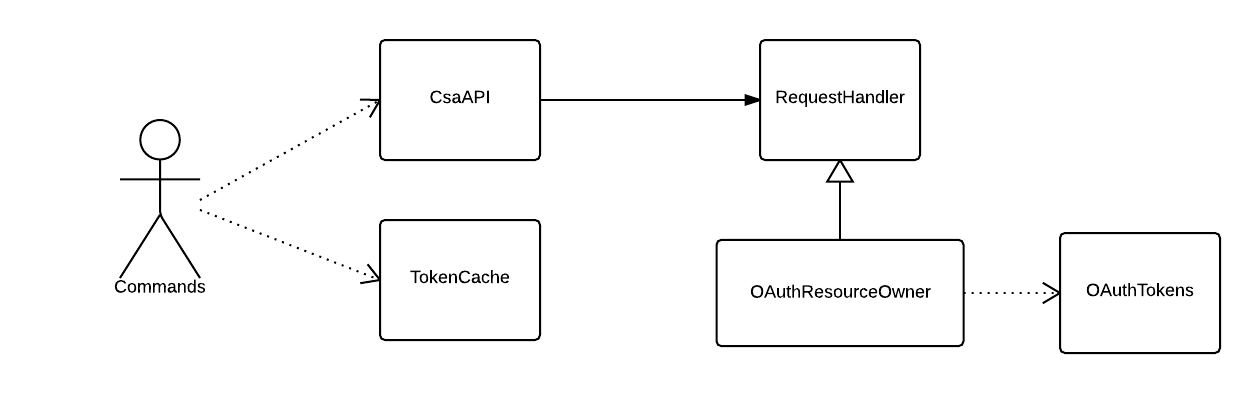
\includegraphics[width=0.8\textwidth]{img/client_class_diagram.png}
\caption{Class diagram for the CS alumni RESTful client application. Note that strictly speaking Commands is not a class but a collection of functions that use instances of CsaAPI and TokenCache.}
\label{fig:client-class-diagram}
\end{figure}

Running a command requires the user to be authenticated with the site. To do this they must first run the authenticate command and supply their user name and password. These details allow the server to generate an access token for the user which can then be used to make further requests to access secure content on the site.

After running a command the access token returned from the server is cached in a local file using the TokenCache class. Internally this class uses the PickleDB library \cite{libraryPickledb} to write out a JSON file. This allows the user to authenticate using their login details just once. The server also issues a refresh token with the access token which is also cached in the file. The access token expires every hour but the OAuthResourceOwner class can automatically handle refreshing the tokens provided that a refresh token is available. When a command other than authenticate is run the OAuth tokens are used. Figure \ref{fig:client-sequence} shows an example ``flow'' of authenticating a user then performing a command.

The CsaAPI class is designed to be used independently of any other classes. In effect it can be used as a stand alone API library for the CSA site. This means that other applications or python scripts can be easily built on top of it without the command line interface. Because each command is executed independently of one another the tokens must be cached to file so that they are stored between runs. If the API was used a part of a different program (such as a GUI) the CsaAPI could be instantiated just once and then multiple calls could then be made without worrying about authentication and token refreshing.

The available commands for the command line application largely mimic the existing functionality and use cases of the original site, along with the same restrictions on operations imposed by the actors in the use cases.

\begin{figure}[H]
\centering
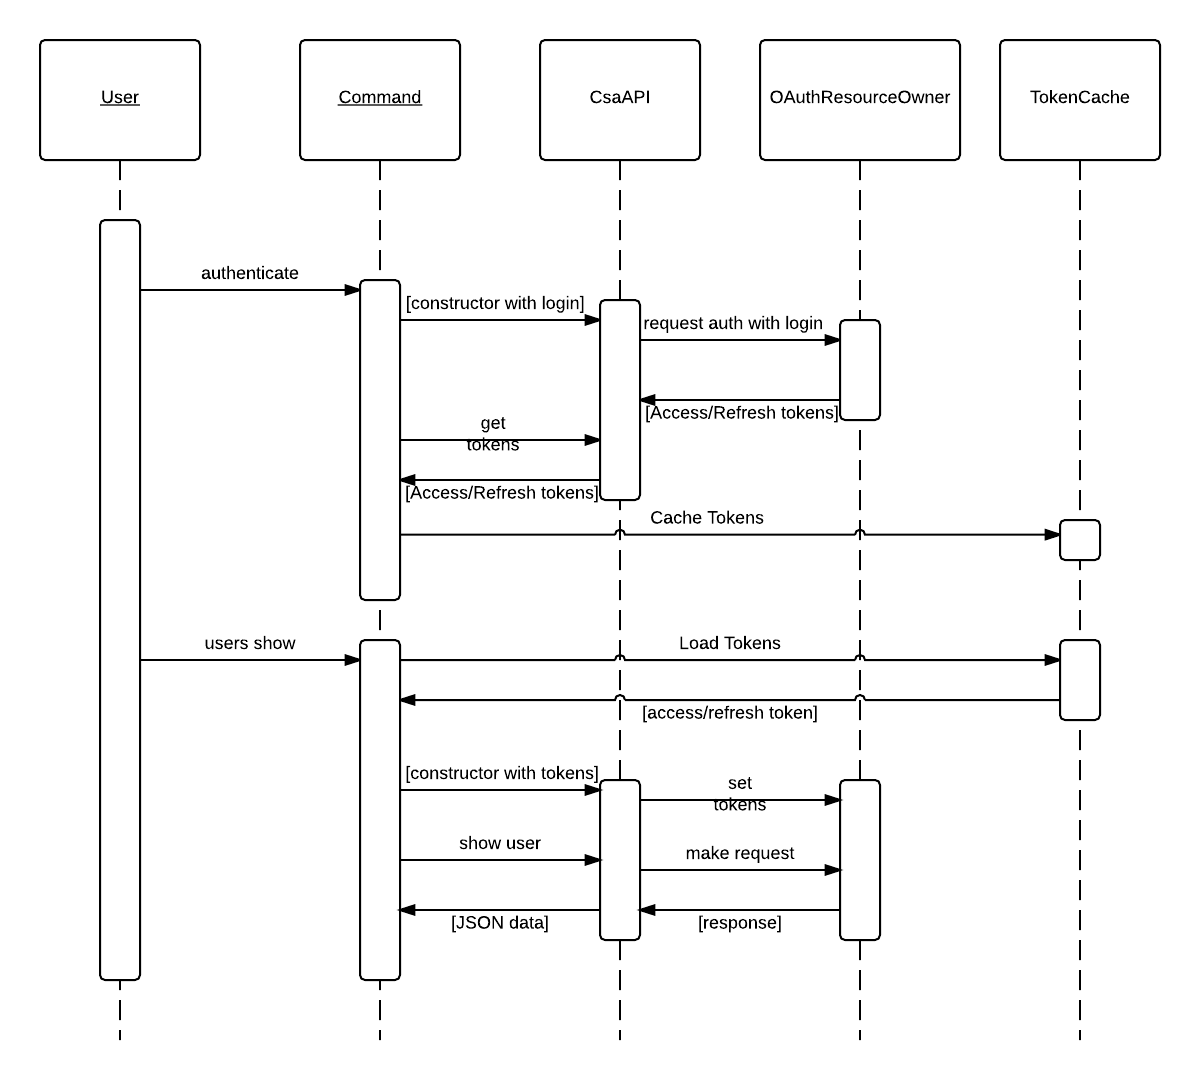
\includegraphics[width=0.8\textwidth]{img/client_sequence.png}
\caption{Sequence diagram for one use case of the client. The client must first authenticate and their access tokens are cached. These tokens are then used to get access to secure data.}
\label{fig:client-sequence}
\end{figure}

\section{Testing}
\label{sec:testing}

\subsection{Testing the Server}
\label{subsec:server-testing}
During the development of this application I attempted to follow a test driven development strategy discussed during the Agile Methodology module of my course. The first thing that I undertook during the development of this project was to bolster the test coverage of the server application. I chose to do this first for threefold reasons:

\begin{enumerate}
\item Writing tests is a exploratory process. It enabled me to explore and understand the existing code base.
\item It provided a safe guard against breaking the server implementation in the future.
\item It ensured that there were no existing bugs in the system which could hinder future development.
\end{enumerate}

I used the SimpleConv gem \cite{librarySimpleConv} to evaluate the current test coverage and provide a target for the number of tests I needed to write. While coverage provides no indication of the quality of the tests running the code, it does show what is currently not being tested at all and is a good baseline of what needs to be done. Generally as a rule of thumb I tried to add both a positive and negative tests for each use case (e.g. can an authorised user edit? Does it fail with an unauthorized user?), and to ensure that both human and machine versions of the site were tested.

\subsection{Testing the Client}
\label{subsec:client-testing}
For the client application I also followed a test driven development approach to testing the application. Supplied alongside the python package I created a folder called tests which contains a test file for each class in the package. As I was starting from scratch with the client application the first thing I did was to write a set of failing tests for the CsaAPI class. As with the server side, I attempted to write both positive and negative tests for each of the use cases. I used the coverage plug-in for the nose library \cite{libraryNose} with the python application to check the coverage level for the program and, as with the server side, use it as a baseline guide check I had enough tests. I also tried to write tests that incorporated the scope of permissions available for both admins and regular users. For example, checking that a user that tries to edit another use causes a 401 error. 

In order to make it possible to run the tests in isolation from the server, I chose to use a HTTP requests mocking library called responses \cite{libraryResponses}. This allowed me to define what the expected response from the server should be independently from the actual server. I used the concept of test ``fixtures'' that Rails uses in my client application by saving some JSON output from the server in local files, then loading them using a test helper function so they could then be used as part of mocked HTTP responses. This worked well to ensure that HTTP requests were being correctly made and that the responses were being processed correctly.

\section{Discussion and Evaluation}
\label{sec:evaluation}
As mentioned in previous sections I attempted to use some of what I learned in the Agile Methodologies module for this course as part of my process for tackling this assignment. I therefore attempted to use test driven development and refactoring instead of developing a concrete design up front. I first researched the libraries that would be most useful in the project (requests, responses, Doorkeeper, click etc.) and made a rough plan of how each of these might be made to hang together. I then focussed on bolstering  testing of the server and writing a test class for the CsaAPI of the client. I then iteratively added more functionality to my project though small pieces of development work focussed on adding particular features (e.g. add support for showing a user).

The thing that worked the best during this project was testing the existing server code base first. This meant I was not likely to break it accidentally, but also got me to read the code and understand how Rails works before blindly hacking away at the code base. It also meant that I got the boring part of development out of the way first and was free to enjoy the more creative aspects of building the client.

While I often felt it hard to stick to at times, I found that the TDD and refactoring approach to development did work for me. Initially my client code started to suffer from the god class anti-pattern, with helper methods for accessing the API and request handing all tied up in one class. However when I started adding OAuth 2.0 support I first started by refactoring the existing code base and quickly found that something like the final design began to ``fall out'' of refactoring. 

I also tried to adhere to the XP principle of YAGNI during development of the client side. I did consider writing the client to use a active record style pattern for data returned from the sever. However considering relative simplicity of the application I decided that this would probably be overkill for the current implementation. If I was developing this further it might be relevant and useful to change the structure to follow such a pattern, but for now I resisted the temptation to use a pattern where it's not needed. Restructuring should be done as and when it's necessary.

One downside I found to following this process was the time it took to write the tests for the application. I feel that the testing I have provided in the client is good but not exhaustive, but it still took me far longer to write half decent tests than it did to actually implement the system. I feel that this was mostly down to the effort of setting up appropriately mocked HTTP responses. Refactoring some of the more common request mocks into test helpers did alleviate this issue somewhat. 

I also had some concerns about the JSON fixtures I was using to test the client becoming out of sync with the actual responses from the server. This was not too much of an issue as I only performed a very small amount of development on the Rails side. However, if I had more changes I anticipate that I would have had many more problems. I think in this case I would of created some integration tests that actually make calls to a version of the server set up with a testing database and I would ensure that the whole process of running the integration tests is automated from start to finish (including setting it up and tearing it down).

Originally, I planned to use an external library called requests\_oauthlib to handle OAuth integration with the CSA site on the client side. However, After spending an entire day making every possible effort to make the client and server talk to each other I eventually gave up using it. The requests\_oauthlib library has only fairly recently added support for OAuth 2.0 and it appears to still be a work in progress. This combined with a lack of documentation on their site meant I was unable to get it working properly. After failing to get it working I decided that the effort involved in getting the resource owner flow of OAuth 2.0 working would not be too difficult so attempted to ``roll my own'' implementation by following the RFC \citep{rfc6749resourceOwner}. I was still able to use the extendible  authentication feature of the requests library to add support for my own implementation which made integrating the code with the existing framework somewhat easier.

On the subject of OAuth 2.0, in the RESTful client I have implemented the resource owner flow which requires the users authentication details to be passed through the client to the site. This is not as secure as the standard, three legged implementation of OAuth because the client must pass their details directly to the (possibly untrusted) client. However the only way to properly implement it is with the use of another server to store the application access tokens as they cannot be communicated to the user through the source code for obvious security reasons. If this were a real site I think it might be appropriate to add support for it, but as the client must install the program directly to their machine we can already assume some degree of trust, along with the fact that it was created by the CSA site maintainer. This also circumvented the extra effort of setting up three legged OAuth which is overkill for such a simple application. This simplification made it easier for me to experiment with OAuth as part of my assignment, something I haven't done before, which was a major learning experience.

Overall, I would award myself 70 percent for this assignment. I feel that I have demonstrated that I can implement a RESTful web service client and maintain an existing project. I feel that what I have done presents a decent effort at testing an application which is not trivial to test. In order to aim for the higher marks I have added additional functionality in the form of very basic OAuth 2.0 support. I feel I have produced a simple and appropriate design that does not force patterns where they are not needed. However, the program is not without its flaws. I could of done something more with integration testing or implemented a three legged OAuth system. There is also no support for image uploads from the command line which would not of been to difficult to achieve if I had more time.

\bibliographystyle{unsrtnat}
\bibliography{references}
\end{document}
